\chapter{Test case}
In questo capitolo è mostato come il linguaggio e l'incarnazione realizzati sono stati applicati ad uno scenario di test noto per quanto riguarda i sistemi multi agente (MAS).
Viene per prima cosa descritto il problema e successivamente analizzati i vari ruoli all'interno della scena.
\\
La soluzione proposta è una ma non l'unica possibile. Una possibile alternativa può esser ad esempio la modifica del modo in cui le pepite sono consegnate. Trasformando il deposito in uno spazio di tuple si dovrà quindi modificare l'azione dell'agente $iSend(R,M)$ sostituendola con $writeTuple(R,T)$, dove $R$ è il destinatario, ovvero il deposito, e la pepita si trasforma da un messaggio $M$ in una tupla $T$.

\section{Descrizione problema}
Il quesito che è stato preso in esame per presentare le funzionalità del progetto sviluppato è noto come `Goldminers' ed è stato definito da Jomi H\"ubner e Rafael Bordini.

\medskip
\fbox{\parbox[t][][t]{1\textwidth}{
In questo scenario un gruppo di agenti minatori deve recuperare pepite d'oro da miniere sparse nell'ambiente e riportarle in un deposito.
}}
\medskip

Il quesito è stato quindi applicato al progetto realizzato in questo lavoro di tesi e sono stati delineati i comportamenti dei ruoli (minatore, miniera, deposito) all'interno della scena: ognuno di essi sarà una specializzazione dell'agente. All'interno di ogni nodo sarà contenuto solo un agente, oltre a quello per il movimento che è `fissato' nel nodo, per via dell'implementazione dell'interprete.
\\
Nella scena gli agenti sono posizionati casualmente all'interno di aree delimitate da cerchi, i quali sono posizionati nell'ambiente secondo le direttive della configurazione. Per ogni tipologia di ruolo è definita l'area del cerchio nel quale sono posizionati gli agenti.
\\
Qui di seguito è descritto come il problema sarà implementato all'interno dell'interprete realizzato.

I minatori conoscono la posizione del deposito: il loro compito è quello di recuperare le pepite e consegnarle al deposito.
Le miniere sono contenitori di risorse, le pepite, che sono estratte dai minatori. Il numero di pepite contenute all'interno di ogni miniera è casuale.

Quando inizia la simulazione i minatori si muovono nell'ambiente alla ricerca di una miniera. Lo spostamento dei nodi viene comandato dall'agente minatore secondo la distribuzione di Levy.
Se il minatore incontra una miniera prova a prelevare una pepita e una volta recuperata la risorsa avvia lo spostamento verso il deposito per recapitare la pepita. Dopo la consegna il minatore riparte verso la miniera da cui ha estratto la risorsa per continuare ad estrarre fino ad estinguerla.
Quando il minatore esaurisce la miniera torna allo stato iniziale, ovvero muovendosi nell'ambiente alla ricerca di nuove miniere da cui estrarre pepite.


\subsection{Tematizzazione della simulazione}
Alchemist nella finestra della simulazione permette di definire degli effetti da applicare ai nodi della simulazione per tematizzarli. La finestra attraverso la quale è possibile definire lo stile è mostrata in Figura \ref{fig:tematizzazioneSimulazione}.

%crea l'ambiente figura;
\begin{figure}[h] % [h] sta per here, cioè la figura va qui
\begin{center} % centra nel mezzo della pagina la figura
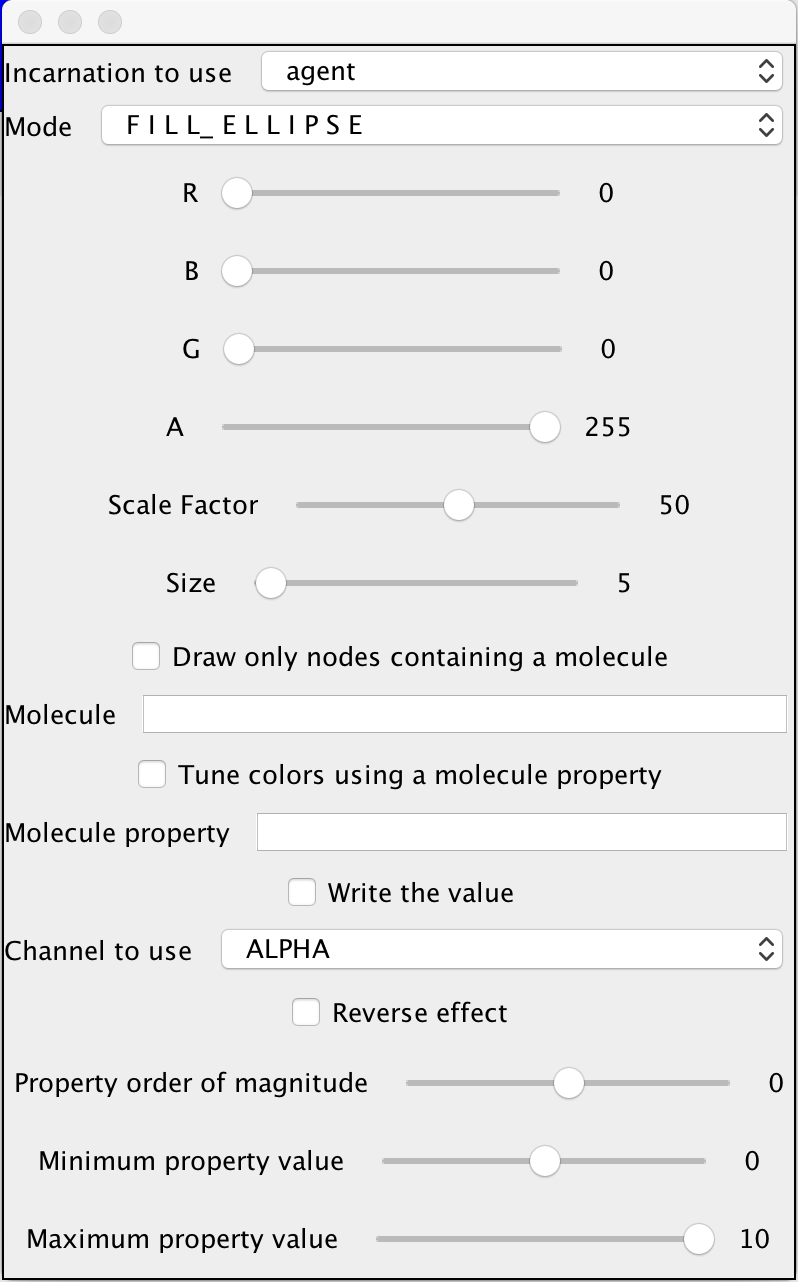
\includegraphics[width=6cm]{images/tematizzazioneSimulazione.png} % inserisce una figura larga 12.5cm
% inserisce la legenda ed etichetta la figura con \label{fig:prima}
\caption[Tematizzazione della simulazione]{Tematizzazione della simulazione} \label{fig:tematizzazioneSimulazione}
\end{center}
\end{figure}

Dall'immagine si può osservare che l'effetto può essere composto da molteplici fattori.
Per quanto riguarda la tematizzazione scelta per questa simulazione sono stati utilizzati i controlli presenti nella prima metà della finestra.
\newline

Sono state definite delle stringhe identificative per le molecole che si riferiscono univocamente ai vari ruoli nella scena: minatore (miner), miniera (goldmine), deposito (deposit), pepita (nugget).
Per stringa è stato creato un relativo stile definito da un colore (tramite il modello RGBA), un fattore di scala e una dimensione per rappresentare il nodo.
\\
L'associazione tra ogni effetto e la rispettiva molecola viene realizzato spuntando la casella di controllo relativa a `Draw only nodes containing a molecule' ed inserendo nella casella di testo sottostante la stringa identificativa della molecola che si vuole abbinare.
\newline

Nell'implementazione dell'interprete sono opportunamente create le molecole utilizzando la classe SimpleMolecule, passando come parametro identificativo le stringhe descritte poco sopra. Gli oggetti istanziati sono poi inseriti all'interno del nodo.

Una volta creato lo stile desiderato è possibile salvarlo (viene generato un file con estensione .aes) in modo da poterlo riutilizzare.
All'avvio di una simulazione di default non è presente nessuna tematizzazione però è possibile caricare un file salvato in precedenza.
La tematizzazione non è necessaria al fine dell'esecuzione della simulazione ma è molto utile per poter comprendere al meglio il comportamento degli agenti nell'avanzamento della simulazione.


\section{Implementazione agenti}
L'agente, come già accennato in precedenza, è composto e definito tramite due parti:
\begin{itemize}
\item la \textbf{teoria} che definisce come e a quali eventi reagire in base ad un contesto;
\item la \textbf{classe} che definisce in che modo i comportamenti sono trasmessi dall'interprete alla teoria.
\end{itemize}
In questa sezione sono descritte le teorie e le classi degli agenti che sono stati implementati per la realizzazione dello scenario di test.

\subsection{Miniera - Goldmine}
La miniera è un'entità che è posizionata in modo casuale all'interno dell'ambiente, che mantiene la sua posizione nel tempo e che contiene delle risorse.
Data questa descrizione la sua realizzazione è stata subito associata agli spazi di tuple. Si è quindi implementata la classe Goldmine estendendo la classe AbstractSpatialTuple.
\\
Per iniziare è stata scritta la teoria dell'agente in cui è definito il suo comportamento e solo successivamente è stata implementata la classe all'interno dell'interprete e le relative funzionalità.

\subsubsection{Teoria tuProlog miniera}
La teoria di questo agente è poco complessa poichè definisce solamente il caricamento di un numero casuale di risorse (ovvero le pepite) sotto forma di tuple all'interno dello spazio di tuple.
\lstset{
  basicstyle=\ttfamily,
  captionpos=b,
  numbers=none,
  frame=tb,
  stringstyle=\color{black}
}
\medskip
\begin{lstlisting}[firstnumber=1,label={lst:Goldmine},caption={Teoria miniera}]
init :-
    agent <- generateNextRandom returns RAND,
    NUGGETS is RAND * 1.0,
    loadNuggets(NUGGETS).

loadNuggets(NUGGETS) :-
    NUGGETS > 0,
    assertz(nugget),
    N is NUGGETS - 1,
    loadNuggets(N).

loadNuggets(NUGGETS) :-
    NUGGETS < 0,
    agent <- setConcentration.
\end{lstlisting}

Nel corpo della regola $init$ viene inizialmente recuperato un numero random, attraverso l'invocazione del metodo $generateNextRandom()$ definito nell'agente, che rappresenta le pepite da posizionare all'interno della miniera.
Il caricamento delle risorse viene fatto tramite l'invocazione della regola $loadNuggets(NUGGETS)$ con la quale sono inseriti i fatti nello spazio di tuple: se le risorse sono state tutte caricate viene invocato il metodo $setConcentration()$,definito appositamente all'interno dell'agente, che viene utilizzato per impostare le molecole per tematizzare graficamente lo spazio di tuple nella simulazione.

\subsubsection{Implementazione classe miniera}
Per quanto riguarda la classe della miniera si è deciso, come detto poco sopra, di utilizzare lo spazio di tuple. La classe astratta AbstractSpatialTuple definisce al suo interno la struttura base dello spazio di tuple e le funzioni per eseguire i suoi comportamenti caratteristici $in$, $rd$ e $out$, rispettivamente trasformati nelle azioni $writeTuple$, $readTuple$, $takeTuple$.
Per definire la miniera è stata quindi definita la classe Goldmine che estende la classe astratta implementando quindi un semplice spazio di tuple.
Oltre ad essere uno spazio di tuple, la classe però implementa anche la super classe astratta AbstractAgent che fa essere Goldmine anche un agente: è quindi necessario implementare all'interno della classe anche i metodi $execute()$ e $cloneAction(node, reaction)$. Il primo di questi due metodi è quello più importante, poichè definisce in che modo lo spazio di tuple opererà nel suo ciclo di ragionamento permettendo a quest'ultimo di reagire alle richieste ricevute.
\\
Per la tematizzazione all'interno della simulazione è stato implementato il metodo $setConcentration()$. Questo metodo, come già accennato nella sezione precedente, viene utilizzato per inserire un oggetto molecola nel nodo, la quale è utilizzata per la tematizzazione della simulazione. La molecola viene creata ed inserita con le istruzioni presenti nel Codice sorgente \ref{lst:CreazioneInserimentoMolecola} solo dopo aver verificato che nella teoria dell'agente sono effettivamente presenti delle risorse.
\lstset{
  numberstyle=\footnotesize\color{black},
  basicstyle=\ttfamily,
  breakatwhitespace=true,
  breaklines=true,
  captionpos=b,
  keepspaces=true,
  numbers=left,
  numbersep=7pt,
  showspaces=false,
  showstringspaces=false,
  showtabs=false,
  tabsize=2,
  frame=tb,
  language=Java,
  commentstyle=\color{gray},
  keywordstyle=\color{blue},
  stringstyle=\color{red}
}
\medskip
\begin{lstlisting}[firstnumber=1,label={lst:CreazioneInserimentoMolecola},caption={Creazione e inserimento molecola}]
SimpleMolecule sm = new SimpleMolecule("nugget");
this.getNode().setConcentration(sm, 0);
\end{lstlisting}
La stringa `nugget' è quella che deve essere inserita nella casella di testo a fianco dell'etichetta Molecule nella Figura \ref{fig:tematizzazioneSimulazione} e che deve essere abilitata cliccando la checkbox appena sopra.
\newline

Per via della necessità di tematizzare la simulazione si è dovuto sovrascrivere il metodo dello spazio di tuple relativo alla funzionalità $out$, o $takeTuple$.
Qui di seguito è descritta la funzionalità già implementata nella classe astratta. Nel paragrafo successivo viene invece riportata la modifica effettuata per definire la tematizzazione della miniera all'interno della simulazione.

Nell'implementazione della funzionalità già definita all'interno della classe astratta, la procedura è la seguente:
\begin{enumerate}
\item recupero di una tupla che corrisponda al template tramite il predicato $retract$;
\item interrogazione per ottenere dal termine estratto il template popolato con i valori recuperati;
\item invio del template popolato tramite un messaggio all'agente che lo aveva richiesto.
\end{enumerate}
Nel caso l'operazione di recupero della tupla non vada a successo quella richiesta viene aggiunta tra quelle in attesa, le quali, se previsto nel ciclo di ragionamento, periodicamente vengono verificate nuovamente per poter essere completate.
Nel caso in cui la richiesta del template è andata a successo e questa è presente nell'elenco di quelle in attesa allora la stessa viene rimossa prima di procedere con l'operazione indicata nell'elenco con il numero 2.

La modifica effettuata è relativa solamente alla tematizzazione, cioè all'inserimento o alla rimozione di un oggetto molecola, e quindi la funzionalità principale rimane quella appena descritta.
Il codice aggiunto è stato inserito prima di effettuare l'operazione di invio del messaggio all'agente. L'aggiunta consiste in un'interrogazione per verificare se dopo aver estratto una risorsa sono presenti ancora pepite, presenti nella teoria sotto forma di fatti, all'interno della miniera. In caso affermativo viene lasciata la molecola che era stata impostata precedentemente invocando dalla teoria la funzionalità $setConcentration()$. Diversamente, se non sono più presenti risorse nella miniera la molecola viene rimossa e, se la tematizzazione della simulazione è opportunamente configurata, il cambiamento porterà ad una modifica dello stile del nodo.

\subsection{Minatore - Miner}
Il minatore è l'agente con il comportamento più complesso per lo scenario preso in esempio.
Il suo compito è quello di muoversi nell'ambiente cercando miniere da cui estrarre risorse da portare al deposito.
Il comportamento del minatore è stato scomposto in 4 fasi o stati:
\begin{enumerate}
\item harvesting: spostamento casuale e ricerca di risorse all'interno di miniere;
\item toDeposit: recuperata la pepita, spostamento verso il deposito per consegnarla;
\item toMine: depositata la pepita, ritorno alla miniera;
\item arrivato alla miniera torna nello stato harvesting.
\end{enumerate}

\subsubsection{Teoria tuProlog minatore}
Le fasi descritte sono state poi riportate all'interno della teoria dell'agente, mostrata nel Codice sorgente \ref{lst:Goldmine}, per definirne il comportamento in relazione agli eventi innescati dall'interprete. Le invocazioni evidenziate in blu sono relative a regole definite all'interno della teoria dell'agente e che non sono state mostrate.
\\
Le regole $ randomDirection(D)$ e $randomSpeed(S)$ restituiscono nella variabile passata, rispettivamente $D$ e $S$, il valore ottenuto dall'invocazione combinata delle funzioni definite all'interno della classe AbstractAgent, e quindi disponibile in tutte le implementazioni di un agente, che generano un valore random e lo applicano alla distribuzione di Levy.
\\
La regola $handlePosition$ si occupa, in modo molto simile a quello che viene fatto nella regola $init$, di generare una nuova velocità e un delta per la direzione da impostare nel nodo, mentre $changeDirection(X,Y)$ modifica solamente la direzione calcolando il valore corretto per raggiungere il punto (X,Y) data la posizione corrente.
\\
La regola $checkMineDistance$ definisce la guardia che verifica che l'agente, dopo aver consegnato la pepita al deposito e essersi diretto alla miniera, è effettivamente arrivato a destinazione e può tornare nello stato `harvesting'.

\lstset{
  basicstyle=\ttfamily,
  captionpos=b,
  numbers=none,
  frame=tb,
  stringstyle=\color{black},
  morekeywords={randomDirection,randomSpeed,handlePosition,changeDirection,checkMineDistance}
}
\medskip
\begin{lstlisting}[firstnumber=1,label={lst:Miner},caption={Teoria minatore}]
init :-
    addBelief(deposit(2,2)),
    addBelief(harvesting),
    randomDirection(D),
    randomSpeed(S),
    node <- changeNodeSpeed(S),
    node <- changeDirectionAngle(D).

%(1)
'<-'(onAddBelief(position(X,Y)), [belief(harvesting)], [handlePosition, takeTuple(nugget)]).

%(4)
'<-'(onAddBelief(position(X,Y)), [checkMineDistance(X,Y,MX,MY)], [removeBelief(mine(_,_)), removeBelief(toMine), addBelief(harvesting), changeDirection(MX,MY)]).

%(2)
'<-'(onResponseMessage(msg(nugget,X,Y)), [removeBelief(harvesting)], [addBelief(toDeposit), addBelief(mine(X,Y)), belief(deposit(DX,DY)), changeDirection(DX,DY)]).

%(3)
'<-'(onAddBelief(distance(deposit,ND)), [removeBelief(toDeposit)], [iSend(deposit,nugget), addBelief(toMine), belief(mine(X,Y)), changeDirection(X,Y)]).
\end{lstlisting}
Nella fase di configurazione iniziale, regola $init$, vengono impostati all'interno della teoria del minatore il belief relativo alla posizione del deposito e quello relativo allo stato iniziale dell'agente, `harvesting'. Successivamente sono generati i valori per direzione e velocità che poi sono impostati nel nodo.
\\
Dopo la regola $init$ sono descritti i fatti che definiscono il comportamento dell'agente, mostrato ad inizio sezione, e che gli permettono di reagire al verificarsi di opportuni eventi.
I fatti seguono la seguente struttura $'<-'(EVENT, GUARD, BODY).$, dove $EVENT$ è l'evento al quale l'agente vuole reagire, $GUARD$ identifica il contesto o la condizione per cui le azioni contenute nel $BODY$ possano essere eseguite.
\\
I fatti identificati dalle fasi 1 e 4 agiscono entrambi in relazione all'evento di aggiornamento della posizione. Il contesto della fase 1 è relativo allo stato `harvesting' mentre quello della fase 4 è la vicinanza del nodo che contiene l'agente rispetto alla miniera che deve raggiungere.
Gli altri due contesti, relazionati ad eventi quali la ricezione di un messaggio dallo spazio di tuple e l'aggiornamento della distanza dal nodo contenente l'agente deposito, sono associati alla rimozione di un certo stato che quindi risulta bloccante finchè lo stato da rimuovere non è presente all'interno della `belief base' dell'agente.
\\
Tra le azioni definite nei corpi dei vari fatti una spiegazione la merita l'utilizzo del belief $mine(X,Y)$. Questo viene utilizzato per salvare la posizione della miniera da cui è stata recuperata l'ultima risorsa, prima di andare al deposito per consegnarla, in modo tale da poter tornare direttamente alla miniera, una volta depositata la pepita, per continuare ad estrarre risorse risultando più veloce ed efficace.

\subsubsection{Implementazione classe minatore}
Per quanto riguarda la parte lato interprete relativa all'agente minatore è stata utilizzata la classe SimpleAgent che estende da AbstractAgent. Questa classe rappresenta un esempio di come può essere immediata l'implementazione di un agente, che racchiude tutte le funzionalità principali, a partire da quello che è già stato prodotto e mostrato precedentemente in questo documento.
\medskip
\begin{lstlisting}[firstnumber=1,label={lst:SimpleAgentReasoningCycle},caption={Ciclo di ragionamento per l'agente completo}]
@Override
public void execute() {
    if (this.isInitialized()) {

        //Agent's reasoning cycle

        this.beliefBaseChanges();

        this.readMessage();

        // SpatialTuples extension
        this.retrieveTuples();

        this.executeIntention();
    } else {
        this.initializeAgent();

        this.initReasoning();
    }
}
\end{lstlisting}
Per implementare la classe SimpleAgent (denominata in questo modo perchè implementa un agente con tutte le funzionalità principali) è stato sufficiente implementare il costruttore, richiamando quello di AbstractAgent, e i due metodi $cloneAction(node, reaction)$ e $execute()$.
Nel Codice sorgente \ref{lst:SimpleAgentReasoningCycle} è mostrato come è stato definito il ciclo di ragionamento.
Come si può notare è stata utilizzata una condizione, che utilizza un flag definito nella classe astratta, per determinare se l'agente è stato inizializzato, ovvero se ha completato la configurazione iniziale.
\\
Nel primo ciclo di ragionamento avviene appunto la configurazione iniziale. La prima funzione che viene chiamata è $initializeAgent()$ che termina la configurazione utilizzata dall'interprete, e all'interno della quale viene modificato il flag citato in precedenza, e poi viene invocata $initReasoning()$ che esegue quanto previsto dalla regola $init$ se presente nella teoria dell'agente.
\\
Dal ciclo di ragionamento successivo vengono eseguite le funzioni per:
\begin{enumerate}
\item controllare le modifiche alla `belief base';
\item leggere i messaggi ricevuti;
\item inviare le richieste agli spazi di tuple;
\item eseguire un'intenzione.
\end{enumerate}
La funzione $beliefBaseChanges()$ recupera tutte le modifiche effettuate alla `belief base' e, per ognuna per cui esiste un comportamento nella teoria, genera un'intenzione inserita opportunamente nella teoria. In modo simile, $readMessage()$ recupera, se presente, un messaggio dalla lista di quelli in entrata e, anche in questo caso, se nella teoria è previsto un comportamento viene generata un'intenzione.
\\
La funzione $retrieveTuples()$ recupera ed invia immediatamente tutte le richieste agli spazi di tuple opportuni.
Per concludere viene invocata la funzione $executeIntention()$ che sceglie un'intenzione tra quelle presenti all'interno dell'agente (il metodo di selezione è Round-Robin), la esegue e poi la inserisce in coda alla lista delle intenzioni.

\subsection{Deposito - Deposit}
Per quanto riguarda il deposito, il suo compito è semplicemente quello di raccogliere le risorse consegnate dai minatori.
Nella soluzione proposta il deposito è stato implementato da un agente ma, come detto nell'introduzione del capitolo, è possibile realizzare simulazioni con un'implementazione diversa.

\subsubsection{Teoria tuProlog deposito}
Per quanto riguarda la teoria del deposito non è necessario definire alcun piano poichè esso non ha compiti se non quello di accettare le risorse ricevute. Si è quindi definita una teoria contenente una regola $init$ vuota (ovvero che ha come unica istruzione del corpo `true').

\subsubsection{Implementazione classe deposito}
La classe utilizzata per rivestire questo ruolo all'interno della simulazione è anche in questo caso la classe SimpleAgent poichè è un'implementazione di un agente completo già pronta per essere utilizzata.
\\
Le funzionalità disponibili sono sicuramente maggiori rispetto a quelle che sono effettivamente utilizzate ma, data la struttura già fornita della classe astratta, questo non impatta sull'efficienza e rimane molto semplice da utilizzare.

\section{Configurazione della simulazione}
Per definire la simulazione si deve scrivere un'opportuna configurazione nella quale sono descritti, attraverso le keyword, quali oggetti utilizzare nella simulazione in relazione al modello creato. Nel Codice sorgente \ref{lst:GoldminersSimulation} sono mostrate e descritte in dettaglio le varie parti che compongono la configurazione e che sono state precedentemente spiegate nella sezione \ref{sctn:ScrivereUnaSimulazione}.

\medskip
\begin{lstlisting}[firstnumber=1,label={lst:GoldminersSimulation},caption={Configurazione simulazione Goldminers}]
incarnation: agent

network-model:
  type: ConnectWithinDistance
  parameters: [2]

displacements:
  - in: {type: Circle, parameters: [2,2,2,0.2]}
    programs:
      -
        - time-distribution: 9
          program: "miner"

  - in: {type: Circle, parameters: [1,2,2,0.2]}
    programs:
      -
        - time-distribution: 9
          program: "deposit"

  - in: {type: Circle, parameters: [1,2,2,0.2]}
    programs:
      -
        - time-distribution: 9
          program: "postman"

  - in: {type: Circle, parameters: [10,2,2,5]}
    programs:
      -
        - time-distribution: 9
          program: "goldmine"
\end{lstlisting}

La prima cosa che si può notare nella configurazione è la specifica dell'incarnazione utilizzata `agent', ovvero quella definita per questo progetto.

Il secondo parametro impostato in configurazione è il `network-model', il parametro che definisce la `linking-rule', che descrive in che modo ogni nodo presente all'interno dell'ambiente è collegato con gli altri. Attraverso questa regola cambia il numero di nodi presenti nel vicinato di ogni nodo. Nel caso specifico, è stato scelto di utilizzare una classe che utilizza la relazione di distanza per collegare i vari nodi ed alla quale è stato passato come parametro il valore 2; per ogni nodo, sono considerati suoi vicini tutti i nodi che ad ogni istante della simulazione siano posizionati all'interno di un cerchio di dimensione 2 il cui centro è il nodo stesso.

Il terzo ed ultimo parametro è `displacements' che definisce una lista con la disposizione dei nodi ed il loro contenuto.
\\
La lista si compone di due keyword: $in$ e $programs$. La prima richiede un oggetto che definisce il tipo della geometria e i parametri per costruirla, mentre la seconda utilizza un'ulteriore lista all'interno della quale sono definite le reazioni associate ad ogni nodo.

Per tutti i ruoli della scena è stato utilizzato il cerchio come geometria per posizionare i nodi, passando per ognuno dimensioni e quantità di nodi differenti.
\\
Attraverso la keyword $program$ si definiscono le reazioni che saranno inserite nei nodi: come si può notare dalla configurazione, per ogni nodo è stata definita una sola reazione.
Per definire una reazione sono stati utilizzati una distribuzione temporale ed una stringa; quest'ultima sarà poi utilizzata durante la creazione di istanze della classe AgentReaction e con la quale verrà istanziata all'interno della reazione la classe dell'agente relativa.
\\
Come parametro della distribuzione temporale è stato scelto 9: questo valore ha consentito, anche in base al valore di distribuzione temporale associato all'azione di spostamento posizionata in maniera intrinseca nel nodo, di avere un comportamento che è sembrato molto fluido.


\section{Metriche di progetto}
Le metriche di progetto rappresentano un insieme di indicatori per tenere sotto controllo e prevedere l'andamento delle principali variabili del progetto (costi, tempi, qualità, risorse).
Le metriche includono solitamente una serie di indicatori standard ma ne possono essere aggiunti altri \textit{ad hoc} in relazione al progetto.
\\
Con le metriche è possibile quantificare in modo obiettivo le performance del progetto misurando gli indicatori predisposti. L'uso principale delle metriche è quello di misurare l'avanzamento del progetto. Il loro utilizzo permette di identificare i problemi di costo/schedulazione prima che diventino criticità e aiutare a focalizzarsi sul completamento delle attività.

\subsection{Metriche software del progetto}
Con le metriche di progetto si misura il codice, quindi è possibile analizzare solamente la parte del lavoro di tesi relativa all'implementazione dell'interprete del linguaggio all'interno del simulatore Alchemist.
La figura \ref{fig:codeMetrics} è stata ottenuta tramite l'utilizzo del plugin CodeMR Metrics disponibile nell'IDE IntelliJ IDEA. Inoltre, è stato utilizzato anche il plugin Statistics per avere un dettaglio maggiore per quanto riguarda le SLOC.
%crea l'ambiente figura;
\begin{figure}[h] % [h] sta per here, cioè la figura va qui
\begin{center} % centra nel mezzo della pagina la figura
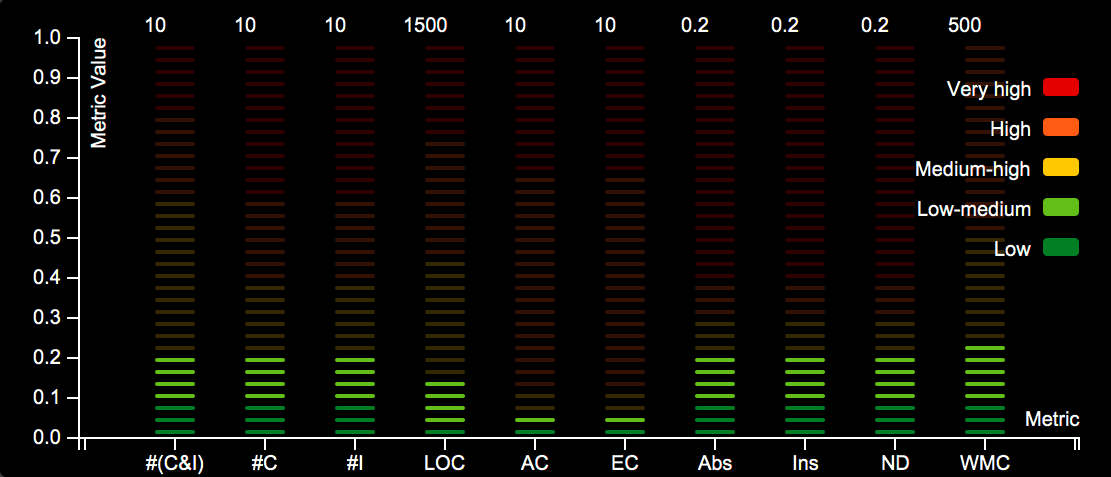
\includegraphics[width=12cm]{images/codeMetrics.png} % inserisce una figura larga 12.5cm
% inserisce la legenda ed etichetta la figura con \label{fig:prima}
\caption[Metriche di progetto]{Metriche di progetto} \label{fig:codeMetrics}
\end{center}
\end{figure}

\medskip
Per la realizzazione dell'incarnazione ad agenti all'interno di Alchemist sono state definite dieci classi Java per implementare la struttura e mostrare come creare le diverse tipologie di agenti. Il totale delle righe presenti all'interno dei file è 2.085, di cui 1.109 sono SLOC e 751 sono di documentazione.
In questo numero non sono calcolate, come accennato precedentemente, le righe scritte per la definizione delle teorie degli agenti utilizzate per la realizzazione degli scenari di test.

La complessità ciclomatica è utilizzata per misurare la complessità di un programma misurando il numero di cammini linearmente indipendenti attraverso il grafo di controllo di flusso.
L'incarnazione realizzata all'interno di Alchemist ha un valore totale di complessità ciclomatica pari a 220, con una media di 2.10.
%crea l'ambiente figura;
\begin{figure}[h] % [h] sta per here, cioè la figura va qui
\begin{center} % centra nel mezzo della pagina la figura
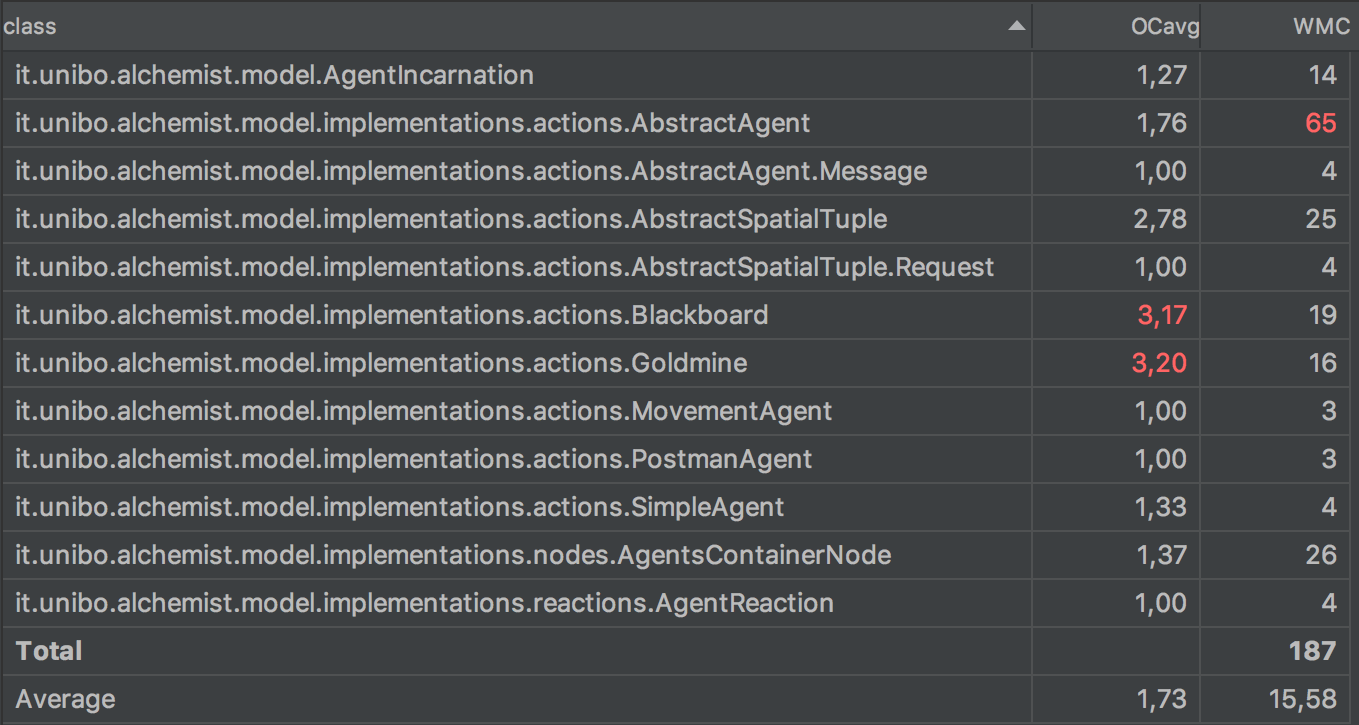
\includegraphics[width=14cm]{images/complessitaCiclomatica.png} % inserisce una figura larga 12.5cm
% inserisce la legenda ed etichetta la figura con \label{fig:prima}
\caption[Complessità ciclomatica]{Complessità ciclomatica} \label{fig:cyclomaticComplexity}
\end{center}
\end{figure}

Nell'immagine \ref{fig:cyclomaticComplexity} è mostrato in dettaglio la complessità ciclomatica delle varie classi, anche quelle innestate, implementate all'interno dell'incarnazione, misurata utilizzando il plugin MetricsReloaded disponibile nell'IDE IntelliJ IDEA. Per ogni classe viene descritto il valore relativo alla complessità operazionale media (OCavg) e quello relativo alla complessità totale(WMC).
La complessità ciclomatica totale dell'incarnazione è 187, la cui media ripartita tra le viarie classi è 15.58.
Si può notare fin da subito che la classe AbstractAgent, la quale definisce tutte le funzionalità di base dell'agente, risulti essere di una complessità ben maggiore rispetto a tutte le altre classi, seguita dalla classe del nodo e poi da quelle che utilizzano il modello SpatialTuples.
Proprio tra quest'ultime, nello specifico Blackboard e Goldmine che sono due implementazioni della classe AbtractSpatialTuple, sono presenti le classi con una compkessità ciclomatica media più alta. Questa caratterizzazione può essere spiegata dal fatto che per definire gli spazi di tuple, vista l'ereditarietà dalla classe AbstractAgent, è stato necessario implementare le funzionalità di gestione dello spazio di tuple, nella classe AbstractSpatialTuple, o nuove personalizzazioni della funzionalità base, nelle implementazioni specifiche degli spazi di tuple.

Per quanto riguarda i metodi presenti all'interno delle varie classi non è mostrato il dettaglio ma sono riportati soltanto i valori totali.
La complessità ciclomatica essenziale, ev(G), è 117, la complessità di design, iv(G), è 213 mentre la complessità ciclomatica totale, v(G), è 220.

